% !TEX root = ../arbeit.tex
\chapter{Software Implementation}
Building a stand-alone \acf{PROCAMS} requires a lightweight and resource saving software. Processing power provided by the ODROID-UX presented in \autoref{sec:sbc} can not stick with current workstations. For a responsive user interface experience, developed algorithms have to be adjusted to the available hardware resources.

As mentioned earlier the ODROID-UX builds on ARM architecture. Linux and Android are natively supported. There continues to be no Windows support for the ARM architecture for researchers. Following a guide\footnote{\url{http://forum.odroid.com/viewtopic.php?f=61\&t=2207\&p=16999\#p16999}}, Ubuntu 12.04 was installed to this relatively new hardware. Some special changes to the video driver and kernel were necessary. Ubuntu was chosen since it is lightweight and has a great library support for different tasks.  
For reading RGB and depth images, OpenNI version 2.2 for ARM \cite{Anonymous:5lF7gVK2} introduced in \autoref{sec:depthSDK} is used. Image processing is done with OpenCV in version 2.4.6 \cite{Intel:H9HpU8rd}. OpenCV is an open source library aiming at real time computer vision algorithms. Visualisation of widgets is accomplished with Qt (version 4.8.2) \cite{Digia:BVAEvJrQ}, a library for UI development using C++ and QML. 

The developed software can be separated into five packages.
\begin{description}
\item[Touch Detection] Detecting direct user input.
\item[Transformation] Mapping of touch events to UI elements.
\item[Pan-Tilt Unit] Receiving user input and controlling pan-tilt unit.
\item[User Interface] Rendering of rectified widgets to surfaces.
\item[Main Logic] Loop handling all events and PROCAMS logic.
\end{description}

\section{Interaction}
Interaction with the PROCAMS is divided into three intuitive parts. First, initial alignment of the projector to create the \emph{interaction space}. In other words where the projection should appear. Secondly placing and arranging the UI-elements namely widgets. And finally, the interaction with widgets itself. The first two tasks are basically one time actions since different alignments of the PROCAMS and the arrangement of widgets are stored. This allows undemanding switching between several surfaces for different use-cases.

The PROCAMS is designed to be ceiling-mounted. Hence, direct manipulation of the alignment is not possible. 
A remote control to control the alignment of the PROCAMS is implemented based on suggested ideas from the interviews. The user is able to control the pan-tilt unit and in this way the alignment of the projection via their smart phone. An Android-App displaying a virtual joystick allows indirect  manipulation as well as storing and loading previous configurations. 

After the configuration of the location, the system executes a self-calibration task. This task is concealed from the user and takes only a short period of time. Then, the PROCAMS can be operated via touch interaction. Following interactions are provided: 
 
\begin{description}
\item[Adding Widgets]  \hfill \\
The user can add widgets by touching and holding the surface at a free spot. A menu with the available widgets appears and the user can choose one of them. The widget is then projected rectified at the previously touched position. Of course, it is possible to add more than one widget to the \emph{interaction space}. 

\item[Moving Widgets] \hfill \\
The user can rearrange the widget by touching and holding (long press) the widget until a red frame appears. When moving the finger around the widget sticks it. When done, the user just presses the green check button and the red frame disappears.

\item[Removing Widgets]\hfill \\
To remove a widget the user long presses on it. When the red frame appears a trash icon on the right side of it needs to be pressed to remove the widget.
\end{description}

After arranging all widgets to the desired layout the user can interact with them immediately. Widgets can offer any content to the user. The current implemented framework forwards four different touch events to the widget. Implemented events are touch down, touch move, long touch and touch release. However, more sophisticated interaction like multi-touch, size and number of touches or the like \cite{Xiao:2013dp} can be easily added to the framework.


\section{Touch Detection}
Accurate and responsive touch detection is a crucial part of this thesis. There are several frameworks \cite{FORTHFoundationforResearchTechnologyHellas:F3nqLAGA,Klompmaker:2012id} and projects \cite{Hardy:2012jo,Xiao:2013dp} supporting finger tracking or touch detection, but all require high performance workstations. Additionally, CUDA (Compute Unified Device Architecture), a parallel computing platform by NVIDIA giving direct access to the GPU processing, or the .NET Framework by Microsoft is required to gain reasonable results. \textcite{FORTHFoundationforResearchTechnologyHellas:F3nqLAGA} developed tracking runs only at 2.67 \ac{fps} on an Intel Core 2 Duo with 2.20GHz and 4096 MBs of RAM using a Quadro FX 1600M for example. Neither CUDA nor .Net is supported by the used SBC. 

For that reasons a unique very lightweight touch detection, based on the research of \textcite{Wilson:2010bv} is developed. A key feature is that touch is detected on any physical object without user driven calibration tasks. 
The developed touch detection can be separated into four parts. First the scenery is analysed and a spatial image, the ground truth, is generated. This obtained image is used to calculate a binary contact image while touch detection is running. The contact image is filtered and simple blob detection detects contact points. In a last step, contact points are tracked over time and transformed into interaction events which finally trigger events intended by the user. 

\begin{figure}[htbp]
        \centering
        \begin{subfigure}[b]{0.31\textwidth}
                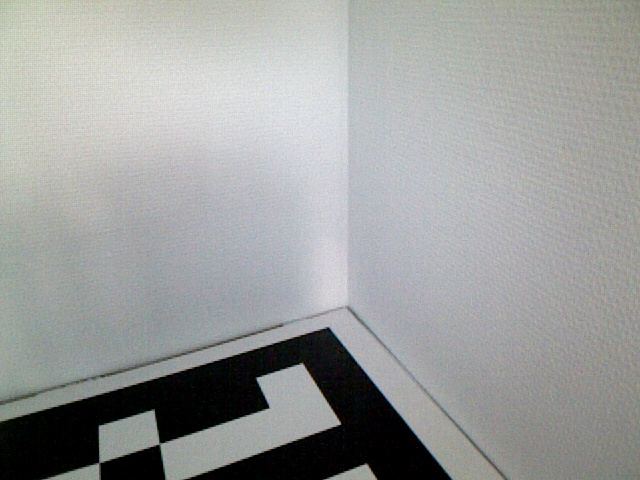
\includegraphics[width=\textwidth]{images/software/gt/RGBImage.jpg}
                \caption{RGB image of scenery}
                \label{img:rgbGT}
        \end{subfigure}
        \hfill
        \begin{subfigure}[b]{0.31\textwidth}
                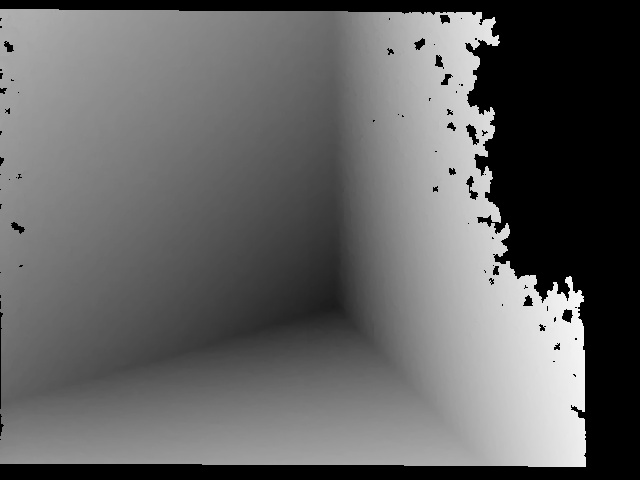
\includegraphics[width=\textwidth]{images/software/gt/actualImage.jpg}
                \caption{Single depth image}
                \label{img:depthGTSingle}
        \end{subfigure}
         \hfill
         \begin{subfigure}[b]{0.31\textwidth}
                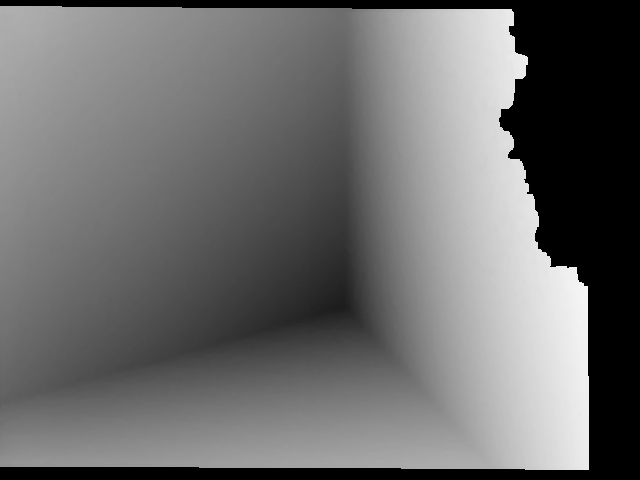
\includegraphics[width=\textwidth]{images/software/gt/GroundTruth.jpg}
                \caption{Filtered ground truth}
                \label{img:GTtemp}
        \end{subfigure}
        \caption{Calculating ground truth}
        \label{img:calcGT}
\end{figure}

The spatial ground truth image is generated by temporal filtering of 30 single depth images. First a dilation operation with a structuring element of 7x7 in size is executed on the depth image. For each pixel depth information is cumulated and divided by the number of depth information available. As result, a good noise reduced approximation of the scenery is calculated. Temporal and spatial filtering is necessary since the depth sensing camera provides only noticeable noisy depth information. A single depth image is shown in~\autoref{img:depthGTSingle} and the corresponding filtered ground truth in~\autoref{img:GTtemp}. Depth information are encoded from near (light grey) to far (dark grey). Black pixel provide no depth information because depth is out of sensing range or because of noise.

A simple assumption is made to enable fast contact image calculation. If the current depth for a pixel is less than the corresponding pixel in the ground truth (minus some offset) and is beyond greater than the ground truth minus the height of a finger, the pixel is representing a potential contact point. This coherence is illustrated in~\autoref{img:finger}. 
\begin{figure}[htbp]
\begin{center}
                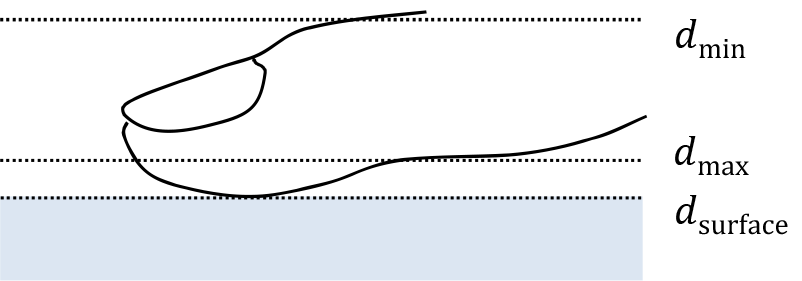
\includegraphics[width=.6\textwidth]{images/software/finger.png}
\caption{Concept of contact point calculation \cite{Wilson:2010bv}}
\label{img:finger}
\end{center}
\end{figure}

Where $d_{surface}$ is the depth in the ground truth image, $d_{max}$ is $d_{surface}-\mathit{offset}$. The $\mathit{offset}$ needs to be well chosen to minimise false positives due to noise. $d_{min}$ is $d_{surface}-\mathit{finger}$. The $\mathit{finger}$ value specifies in which height from the surface a contact is detected. Mathematical a pixel $d(x,y)$ is a potential contact point if the following formula holds:
\begin{equation*}
d_{max}(x,y) > d(x,y) > d_{min}(x,y)
\end{equation*}

A contact point image is illustrated in~\autoref{img:cpT}. Since there are still some false positives the image needs to be filtered before a blob detection can be executed. Therefore a low-pass 3x3 box filter and subsequent thresholding is applied. 
For performance reasons the box filter is separated into one 1x3 respectively 3x1 filter. Separating the filter leads to faster filtering by more than 40\%. A filtered contact point image is shown in~\autoref{img:fcpT}
On this filtered image a blob detection is executed. First the \textit{SimpleBlobDetector} of the OpenCV framework was applied, but it proved to be too slow. Analysing one frame takes between 45 and 58 ms which is far from realtime. Hence, an alternative library namely OpenCVBlobsLib\footnote{\url{http://opencvblobslib.github.io/opencvblobslib/}} is utilised. This library makes use of multi core processing and analyses an image in less than 6ms. The result of a blob detection is illustrated in ~\autoref{img:rgbT} and~\autoref{img:blobdetectT}. Detected blobs are marked green in these images.

\begin{figure}[htb]
        \centering
        \begin{subfigure}[b]{0.48\textwidth}
                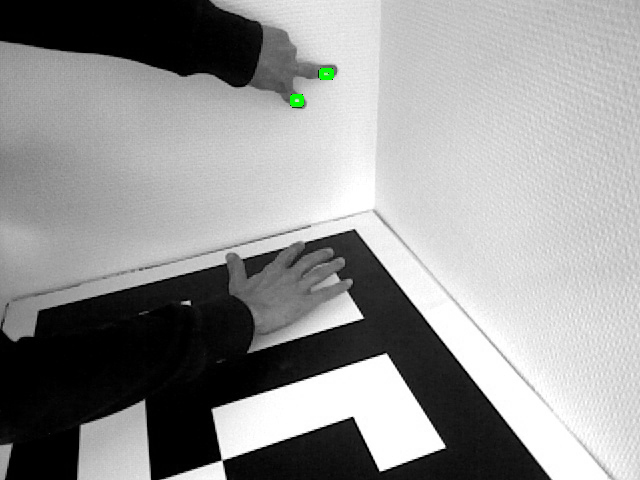
\includegraphics[width=\textwidth]{images/software/no_touch/RGBImage165644_comob.jpg}
                \caption{Image with detected touch points}
                \label{img:rgbT}
        \end{subfigure}
    \hfill
        \begin{subfigure}[b]{0.48\textwidth}
                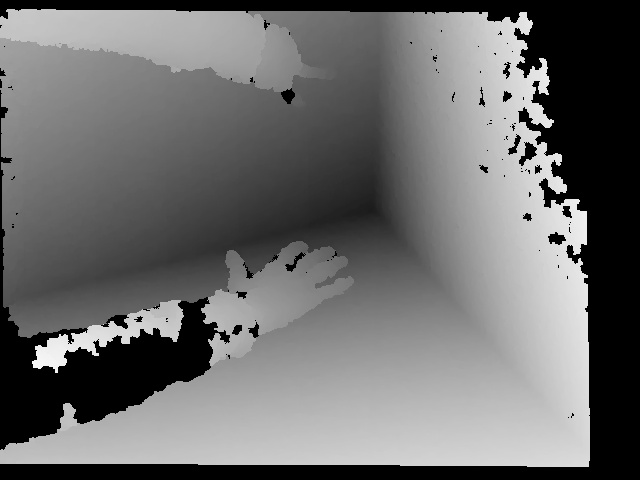
\includegraphics[width=\textwidth]{images/software/no_touch/actualImage.jpg}
                \caption{Depth image for touch detection}
                \label{img:depthT}
        \end{subfigure}        
               
      \vspace{1em}

        \begin{subfigure}[b]{0.31\textwidth}
                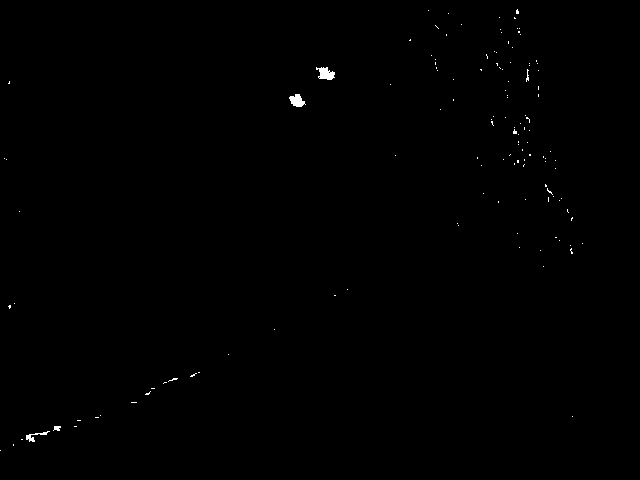
\includegraphics[width=\textwidth]{images/software/no_touch/initalDiffImage.jpg}
                \caption{Potential contact points}
                \label{img:cpT}
        \end{subfigure}
     \hfill
        \begin{subfigure}[b]{0.31\textwidth}
                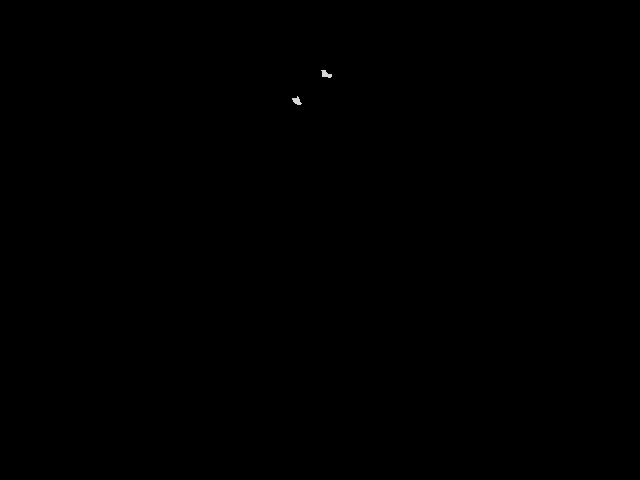
\includegraphics[width=\textwidth]{images/software/no_touch/filteredDiffImage.jpg}
                \caption{Filtered contact points}
                \label{img:fcpT}
        \end{subfigure}
        \hfill
         \begin{subfigure}[b]{0.31\textwidth}
                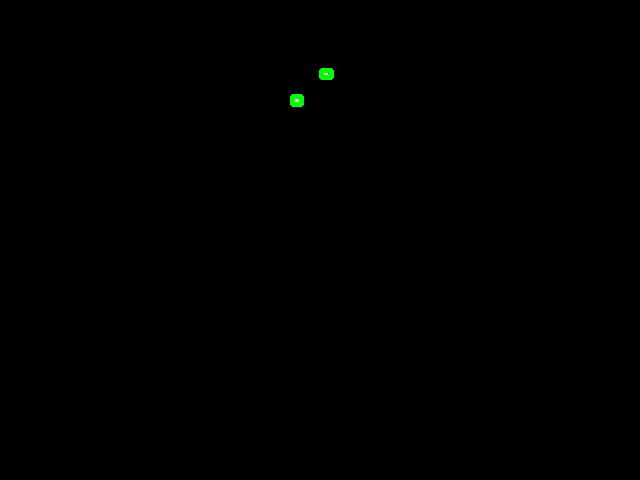
\includegraphics[width=\textwidth]{images/software/no_touch/blobs.jpg}
                \caption{Detected blobs}
                \label{img:blobdetectT}
        \end{subfigure}
        \caption{Touch detection sequence showing two touching fingers and one hovering hand.}
        \label{img:calcGT}
\end{figure}
Due to the prior analysis of the scenery, contact points can be detected on any random shaped surface as long as the depth sensing camera can see it. This allows in particular simultaneous touch detection on diverse aligned surfaces. 

Detected contact points are tracked over time to classify them into different touch events. As described prior events are touch down, touch move, touch release and long touch. The implemented tracker assigns the $\mathit{time}$
of the first appearance, $\mathit{age}=0$  and $\mathit{lives} = 5$ to each new detected blob. In subsequent frames distances between previous blobs and the new blobs are calculated. If the distance is below a certain threshold, the $\mathit{age}$ for this particular blob is increased. Additionally, the distance is cumulated and stored in $\mathit{movement}$. This is used for long touch detection.  
For all previous blobs, where no corresponding blob is found, the $\mathit{lives}$ is decreased. All new blobs are handled like described before. Touch events are differentiated as following: 

\[
    \mathit{event}= 
\begin{cases}
    \text{touch down},& \text{if }  \mathit{age} = 3 \\
    \text{long touch}, & \text{if } \mathit{age} > 3 \wedge \mathit{movement}<\mathit{thld}_{move} \wedge \mathit{time}_{elapsed} =  {thld}_{time}\\
    \text{move}, & \text{if } \mathit{age} > 3\\
    \text{touch release},& \text{if } \mathit{age}  \geq 3 \wedge \mathit{lives} =0\\   
    \text{no event},& \text{otherwise}
\end{cases}
\]
Where $\mathit{thld}_{move}$ is the threshold for the maximum allowed distance the finger can drift whereby a long press is still detected and $\mathit{time}_{elapsed}$ is the time a long press takes.

The position of a touch event is detected in the depth sensing camera coordinate system. Whereas all \ac{GUI} elements also known as widgets are located in the projector coordinate system. Hence, event coordinates need to be transformed to the projectors coordinate system. This transformation procedure is outlined in the next section.

\section{Calibration and Transformations}
Mapping the detected touch event coordinates from the camera coordinate system to the widget, displaying the content, is necessary to enable interaction at all. Therefore, the touch event point $P_{x,y}$ detected in the camera coordinate system is transformed several times until the point is located in the same coordinate systems as the widget. In detail, the touch point is transformed from the depth sensing camera coordinate system to the colour camera coordinate system. From there to the world coordinate system which is the only three dimensional coordinate system in the transformation process. From the world coordinate system, the point can be transformed to the projectors coordinate system. There it is transformed one last time to the widgets coordinate system since it is pre-warped. This many transformations are indispensable because only the transformation matrixes between the named coordinate systems are known or can be determined due to manual one time calibration task.

\subsection{Camera-Projector Calibration}
The most challenging part is to determine the transformation between the depth sensing coordinate system and the projectors one. \textcite{Xiao:2013dp} present an approach to determine the perspective transformation between a Kinect and a projector, but a special 3D-calibration target is needed. Hence, such a target was not accessible other approaches were evaluated. 
Simple colour-camera-projector calibration algorithms are developed by \textcite{LegardaSaenz:2004hn,Gao:2008jn,Li:2008kr} using structured light or \textcite{Ashdown:2005dx,Griesser:2006ko,Audet:2009ee} using optical pattern.

Using the colour camera for camera projector calibration requires to transform the touch point from the depth sensing coordinate system to the one of the colour camera. Despite that, an additional concept for calibration presented by~\textcite{Audet:2009ee} was chosen. Especially because he provides a software, ProCamCalib\footnote{\url{http://www.ok.ctrl.titech.ac.jp/~saudet/research/procamcalib/}}, which performs a ``full calibration of a camera and a projector in about 30 second'' by preserving comparable good results as the preceding stated concepts. 

To use the ProCamCalib software a special \textit{framegrabber} was implemented since the software was originally developed for simple web-cameras and not for depth sensing cameras. The OpenNI framework was used to read colour frames from the PrimeSense camera. The frames were then transformed in a ProCamCalib readable format.

\begin{figure}[htbp]
        \centering
        \begin{subfigure}[b]{0.486\textwidth}
                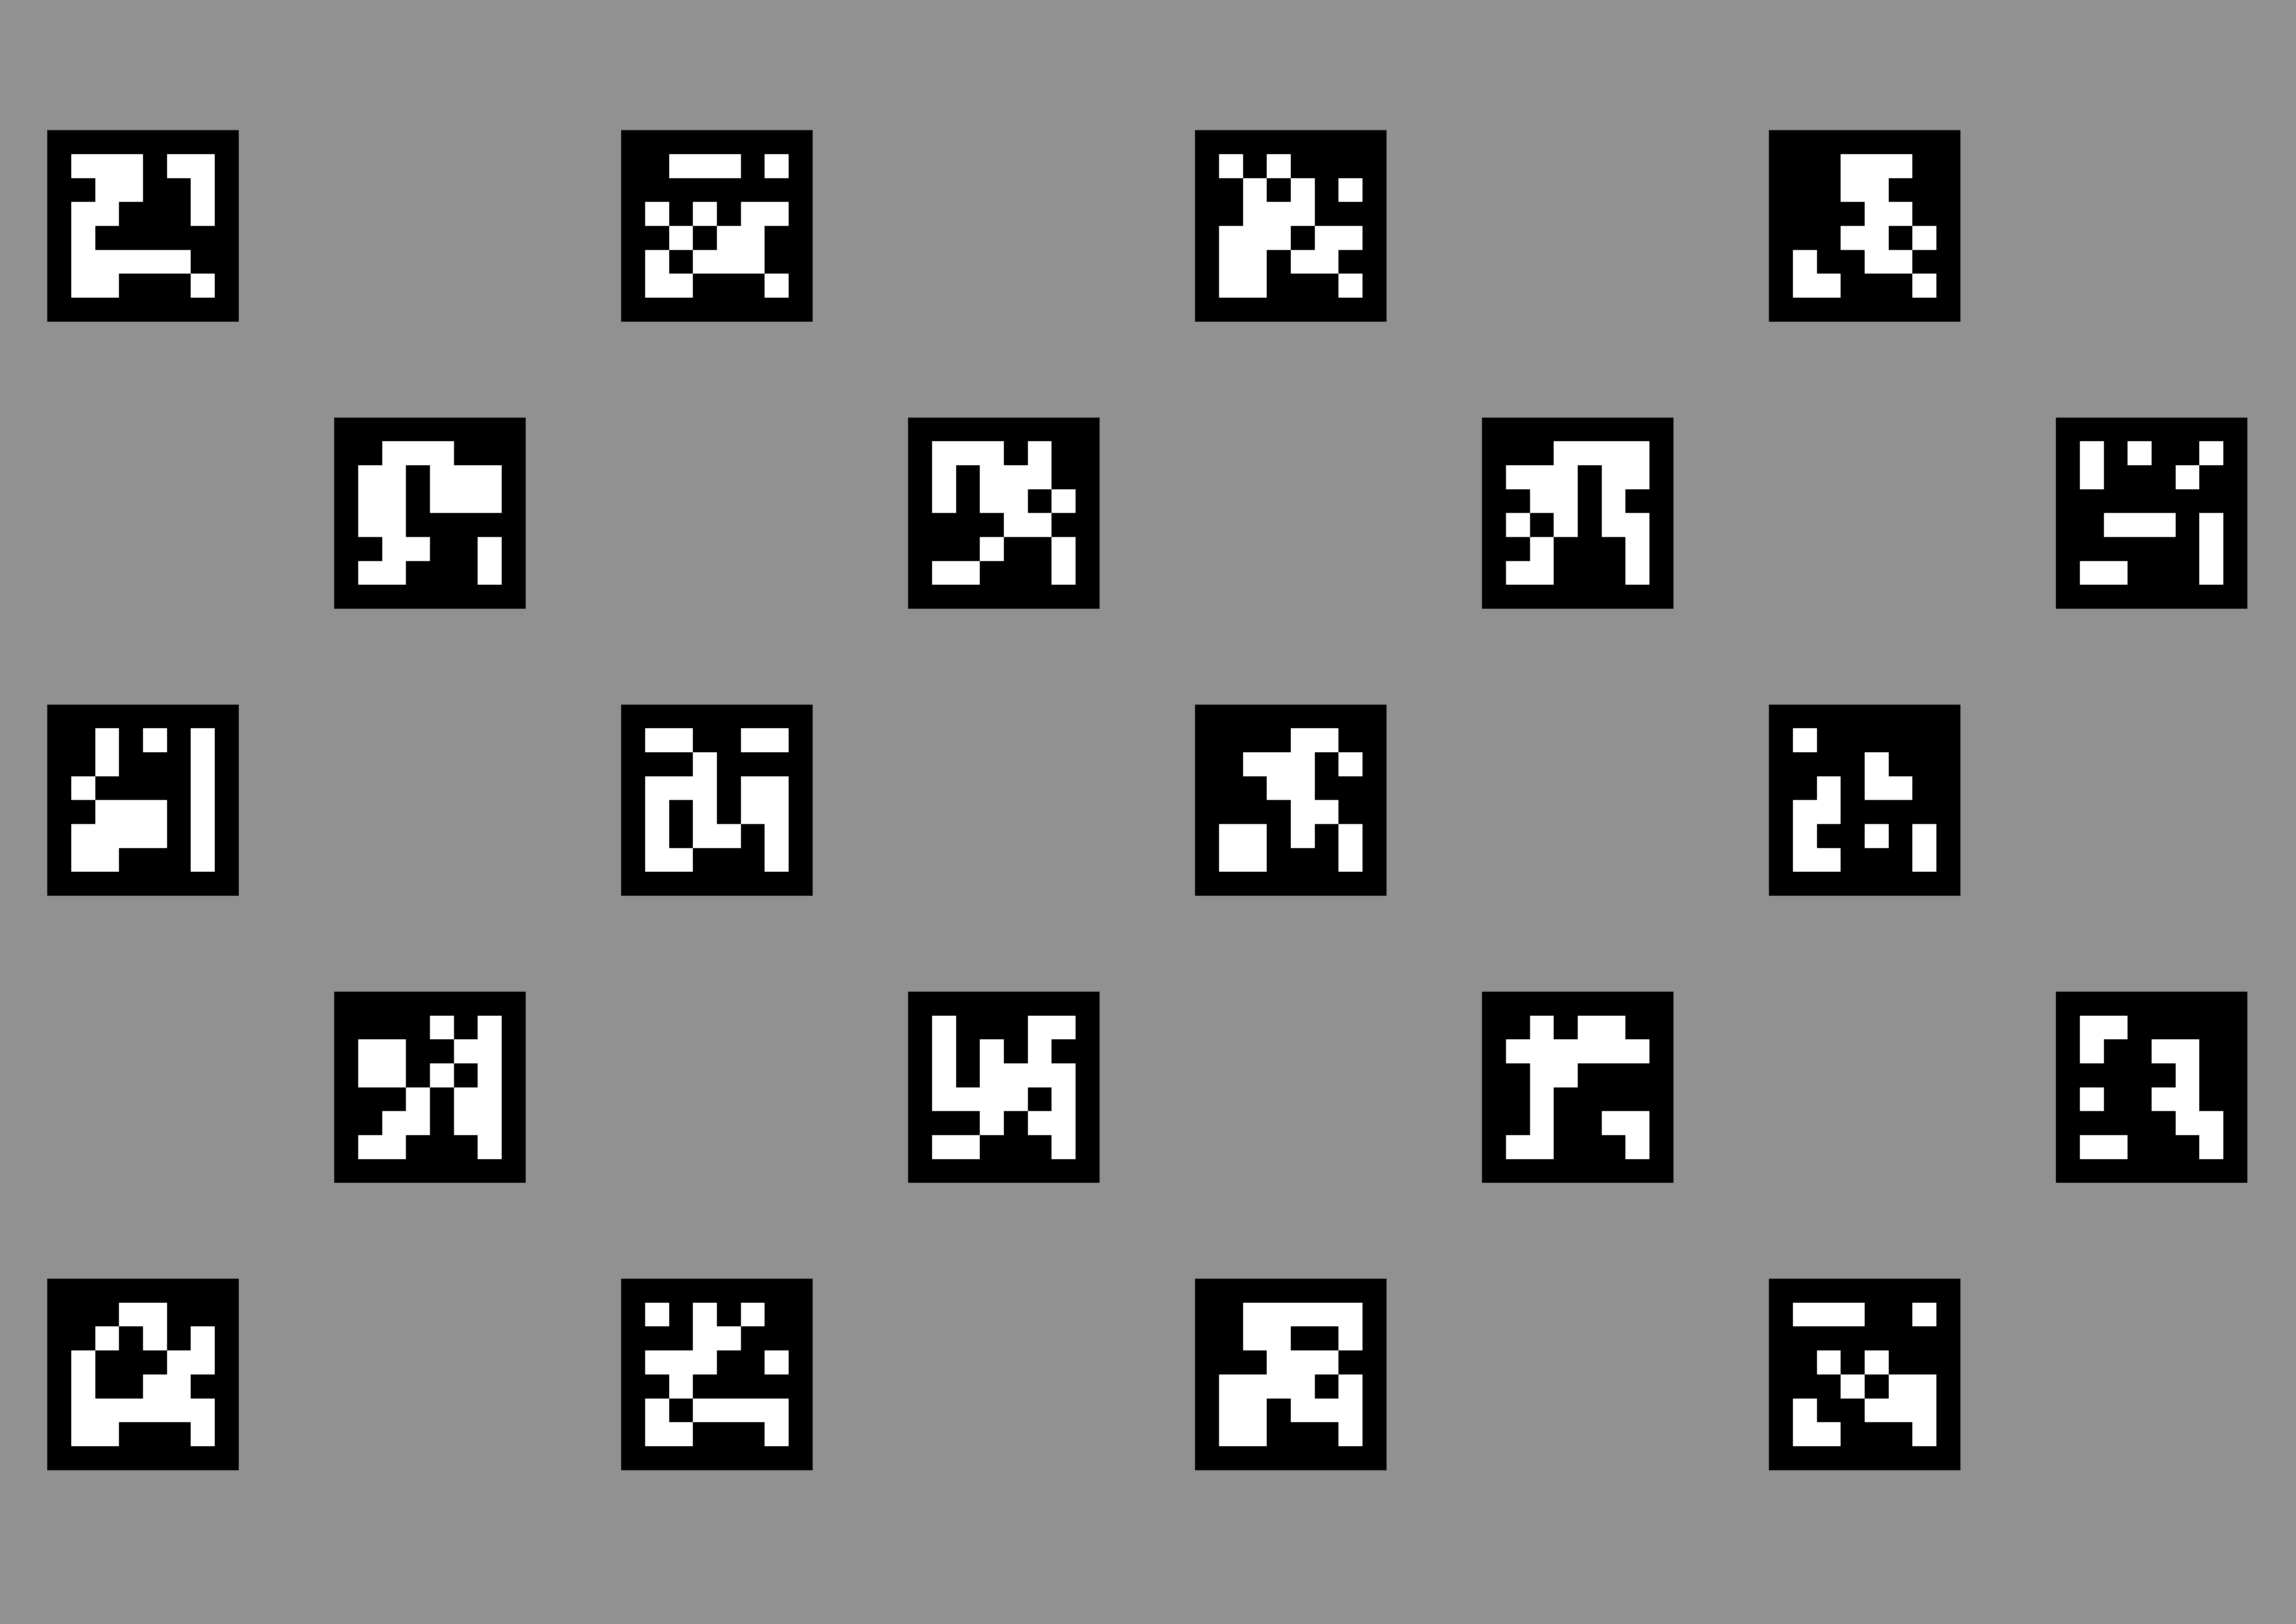
\includegraphics[width=\textwidth]{images/software/barcode.png}
                \caption{Printed barcode pattern}
                \label{img:patternCalib}
        \end{subfigure}
    \hfill
        \begin{subfigure}[b]{0.46\textwidth}
                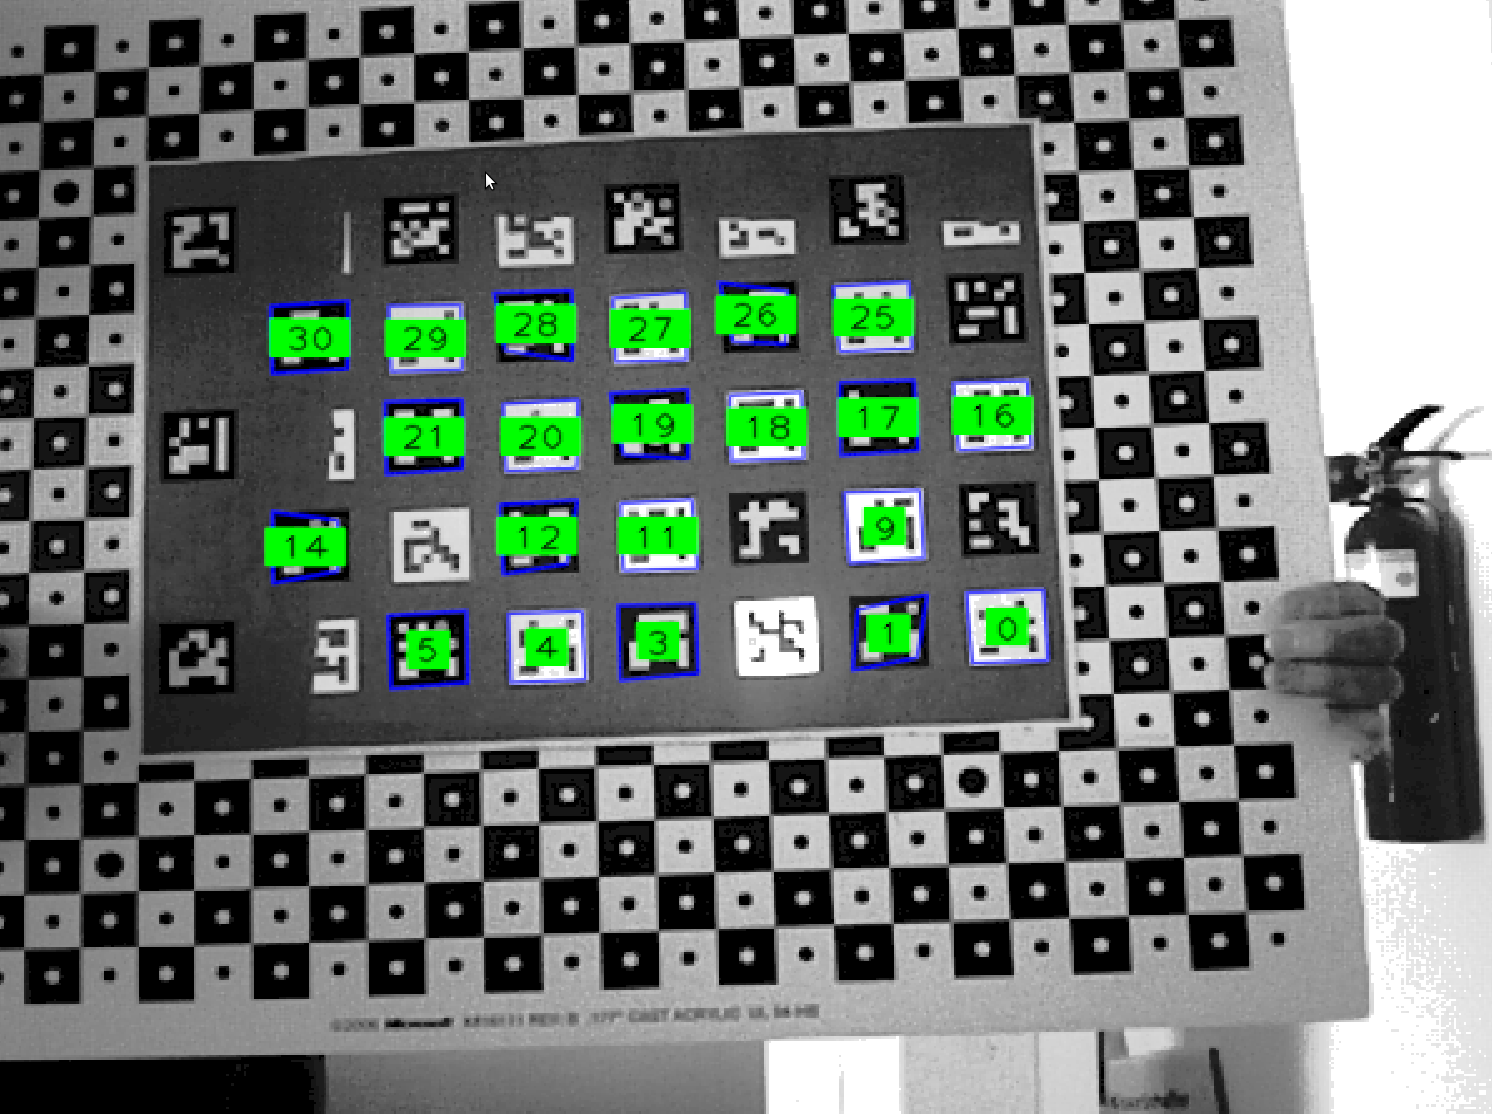
\includegraphics[width=\textwidth]{images/software/calib.png}
                \caption{Calibration process}
                \label{img:calibCam}
        \end{subfigure}        
        \caption{Projector camera calibration with printed and projected barcode pattern}
        \label{img:calibrationproces}
\end{figure}
Indeed, the calibration task itself is really simple. The printed pattern containing fiducial markers (shown in~\autoref{img:patternCalib}) enables the software to calculate the intrinsic parameters of the camera. Then the projector starts to project an inverted  marker pattern into the spaces of the printed one which the camera tries to recognise (see~\autoref{img:calibCam}) simultaneously. The intrinsic parameters of the projector can be calculated when the projected pattern is detected. Knowing this information the software takes several pictures showing the pattern in different poses and calculates the extrinsic parameters which reflect the relation between the camera and the projector. With this information touch points can be transformed from the camera coordinate system into the 3D world coordinate system and then into the projectors one. The calculated calibration file for the built PROCAMS is printed in~\autoref{apx:calib}.

\subsection{Transformation}
As mentioned, several transformations are necessary to calculate the position of the touch event represented in the widgets coordinate system. In the following, the executed transformations are described in detail. 

\subsubsection{Depth Sensing Camera - Colour Camera}
The transformation between depth sensing camera and colour camera is necessary since the calibration was performed between colour camera and projector. Fortunately, the OpenNI framework in combination with the used PrimeSense camera allows a direct mapping of the depth sensing camera image to the colour camera image. This is done internally by the camera hardware so no computational performance is wasted. 

\subsubsection{Colour Camera - World}
The $3\times4$ camera matrix describes the mapping from 3D points in world space to 2D points in a camera image. It is identified in the calibration task. Using the inverse camera matrix as well as the camera distortion coefficients which contains the intrinsic parameters allow in combination the distance from the depth sensing camera a retransformation of the touch point into the 3D world coordinate system. For matrix multiplication and rectification, OpenCV library is used. 

\subsubsection{World - Projector}
Transforming the point from the  3D world coordinate system into the projector space is the inverse operation to the colour camera - world transformation using the projectors parameter. This time the projector matrix containing the alignment of the projector in the world coordinate system as well as the projectors distortion coefficients are used to calculate to perspective projection of the 3D point onto the projector image. This operation is also performed using the  OpenCV library. 

\subsubsection{Projector - Widget}
Since the widget is pre-warped to enable a rectified projection the touch point needs to be transformed once again.
The transformation of the widget is set out in~\autoref{sec:widget}. Since the perspective transformations matrix which is applied to the widget is known, the touch point can be transformed in the same manner. 

Finally, the coordinate of the touched point is known and the interaction can be performed as designated by the widget. 
	
\section{Pan-Tilt Unit Control}
\begin{wrapfigure}{r}{0.5\textwidth}
		\vspace{-2em}
  		\begin{center}
                	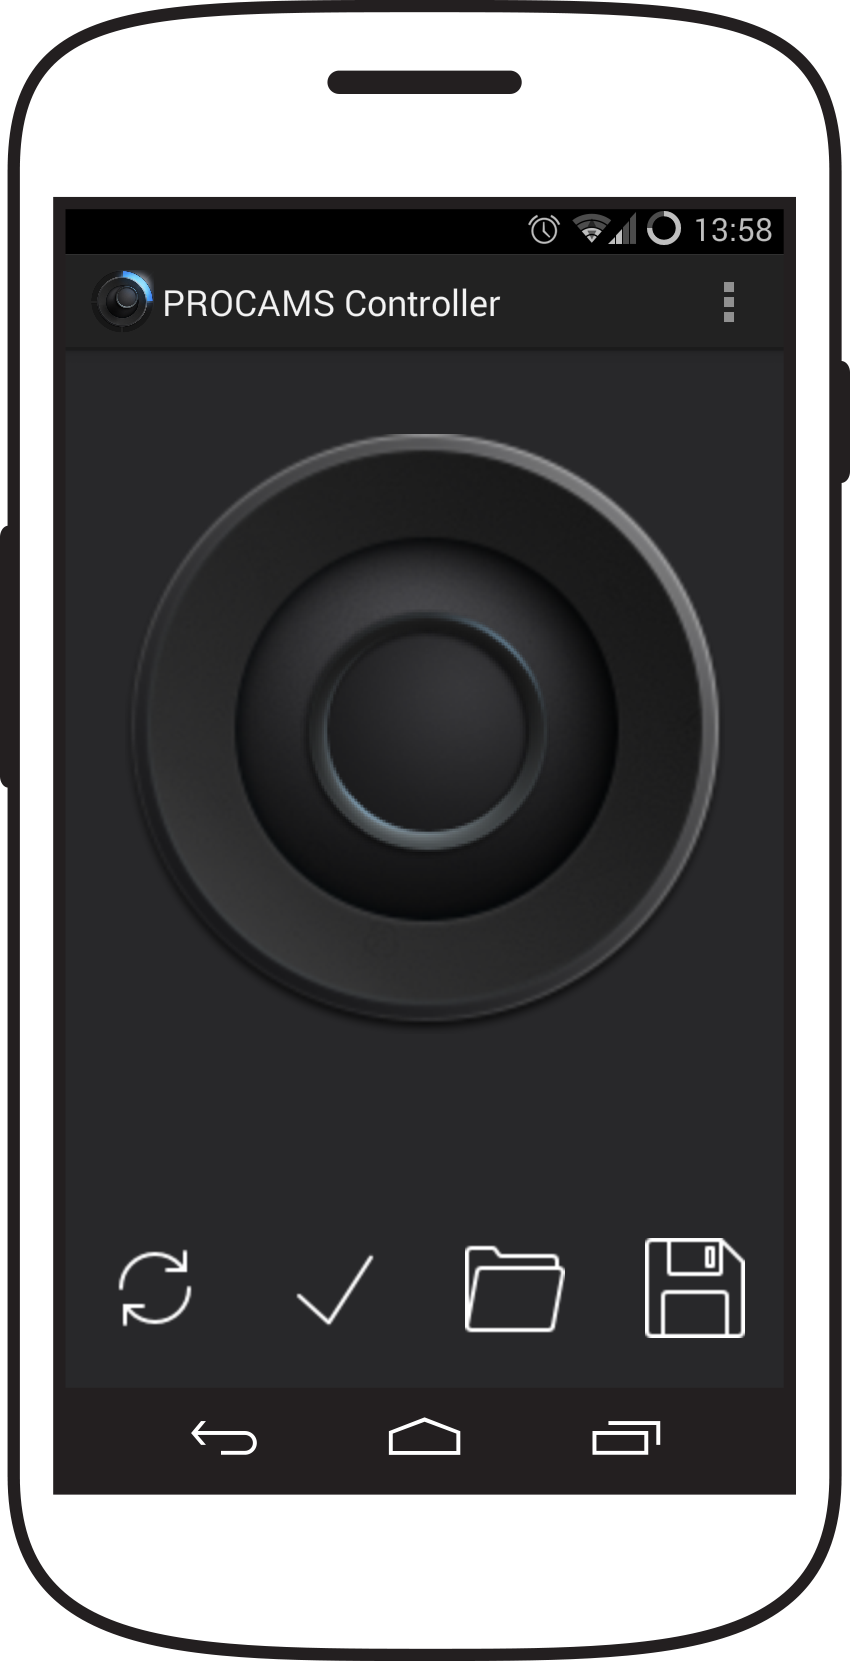
\includegraphics[width=.42\textwidth]{images/software/android_template.png}
  		\end{center}
		  \vspace{-1em}
		  \setcapindent{0pt}
		  \captionsetup{width=0.42\textwidth}
\caption{Android App providing control over the PROCAMS pan-tilt unit via joystick}
	\label{img:appUi}
       \vspace{-3em}    
\end{wrapfigure}

The user can execute the initial alignment of the PROCAMS remotely. An Android App was implemented to provide basic control of the pan-tilt unit. The App UI is shown in~\autoref{img:appUi}. It consists of a virtual joystick and four buttons for storing and loading surface configurations as well as starting interaction and recalibrating. Moving the joystick on the display triggers the pan-tilt unit to move the PROCAMS to the desired direction. Meanwhile, the projector is rendering a frame indicating the resulting \textit{interaction space}

The App connects via Internet to the server running on the PROCAMS. The server receives the movement commands (up, down, left, right) and forwards them via serial interface to the connected Arduino microcontroller which handles the movement of the servos. The check button triggers the self-calibration task for the touch detection and starts the system for user interaction. The recalibrate button provides the opportunity to repeat the calibration task if for example the touch detection ground truth run out of sync due to unintentional movement of the PROCAMS. Pressing the store button asks the user to provide a name for the current configuration. The store command and the name are then transmitted to the server which stores name, current position of the PROCAMS as well as the position of the widgets in a database. On pressing the load button all stored positions are loaded from the server and displayed to the user for selection.

\section{User-Interface} 
After setting up the alignment of the PROCAMS and self-calibration of the touch detection is done the user can start placing widgets. The interaction space is still indicated by a light white frame.

The projector is usually not aligned perpendicular to the surface it is projecting to. This causes geometrical distortion. 
Rendering a representation of the widgets without distortion onto the surfaces requires a pre-warping according to the alignment of the projector to the surface.


\subsection{User-Interface Pre-Warping}
For the proposed PROCAMS, the already available depth map, the ground truth calculated for touch detection, is used to facilitate a rectified projection. First a plane detection is executed on the depth map to find possible projection surfaces. Then four points situated on one of the detected planes, spanning a rectangle of the desired size are determined. Finally, the affine transformation which transforms the widget to the determined points is calculated and applied to render a corrected representation of the widget. These three steps will now be described in detail.

\paragraph{Plane Detection} 
Plane detection is done following the concepts \textcite{Yoo:2013he} presented in their work. To compute the surface normal of a point $P_{x,y}$ in the ground truth depth map, four points with a distance $d$ around the point are selected. Up: $P_{x,y-d}$, Down: $P_{x,y+d}$, Left: $P_{x-d,y}$ and Right: $P_{x+d,y}$. $d$ defines the amount of smoothing. A greater $d$ will flatten the surface normal since it is calculated over a larger area. These four points are transformed into world space and the vectors between up-down and left-right are determined (see~\autoref{img:normalsCalculation}). The cross product of these two vectors is finally the surface normal $N_{x,y}$ of the point $P_{x,y}$.

\begin{figure}[htpb]
        \centering
        \begin{subfigure}[b]{0.31\textwidth}
	      \centering
               \def\svgwidth{.78\textwidth}
               \import{images/software/ui/}{dmap2.pdf_tex}
                \caption{Surface normals calculation scheme \cite{Yoo:2013he}}
                \label{img:normalsCalculation}
        \end{subfigure}
         \hfill
                  \begin{subfigure}[b]{0.31\textwidth}      
                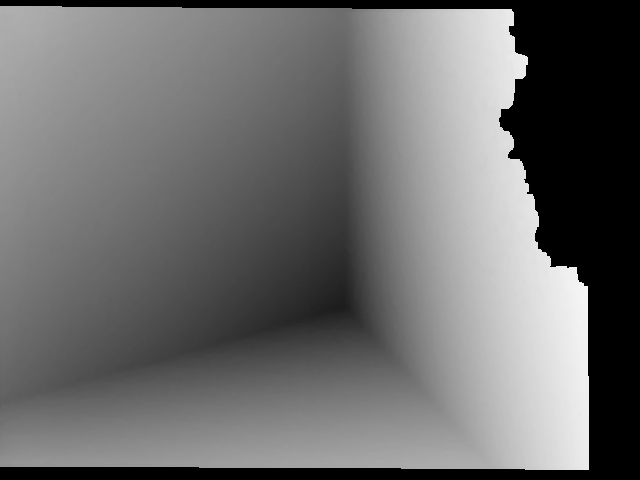
\includegraphics[width=\textwidth]{images/software/gt/GroundTruth.jpg}
                \caption{Depth map of scenery\newline}
                \label{img:normalGT}
        \end{subfigure}
         \hfill
         \begin{subfigure}[b]{0.31\textwidth}      
                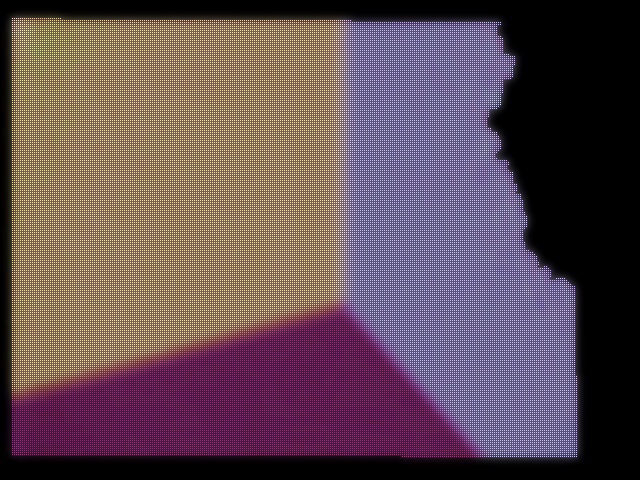
\includegraphics[width=\textwidth]{images/software/gt/normalsImage_mod_2.jpg}
                \caption{Colour encoded surface normals}
                \label{img:normals}
        \end{subfigure}
        \caption{Plane detection}\label{fig:animals}
\end{figure}
Surface normals are directly calculated after determination of the ground truth in the self-calibration task. To minimise processing time surface normals are only calculated over a grid with a distance of 4x4 pixel. For a given ground truth like illustrated in~\autoref{img:normalGT} the corresponding surface normals are presented in~\autoref{img:normals}. The length of each direction (X,Y,Z) of the normal vector $N_{x,y}$ is encoded via a corresponding colour (red,green,blue). Hence, surface normals pointing in the same direction have the same colour. 


\paragraph{Rectangle Calculation}
When the user presses long at the surface to add a new widget, the position as well as the surface normal in camera-space is known. 
Both define a plane where the widget should appear rectified. Therefore, the plane (point and normal) is transformed into world space. Based on the normal vector, two vectors $x$ and $y$ each perpendicular to each other and to $N_{x,y}$ are calculated. Hence the alignment of the pan-tilt unit is known $x$ and $y$ can be rotated in that way, that $y$ points down and $x$ is horizontal  in the 3D coordinate system. The calculated vectors are displayed in red and blue in~\autoref{img:vectors}. 

\begin{figure}[htpb]
        \centering
               \def\svgwidth{.35\textwidth}
               \import{images/software/rectify/}{surface_2text.pdf_tex}
                \caption{Surface normals calculation in world-space}
                \label{img:vectors}
\end{figure}
Knowing the two vectors, allows to calculate the four vertexes of the rectangle where the widget should appear. 
The four points can be calculated as follows:

\begin{equation*}
\begin{split}
\text{P}_0 & = P_{x,y} \\
 \text{P}_1 & = P_{x,y} +w\times x  \\ 
\text{P}_2 & = P_{x,y} + h\times y \\
 \text{P}_3 & = P_{x,y} + w\times x + h\times y   \\ 
\end{split}
\end{equation*}

Where $P_{x,y}$ is the point the user touched, $w$ the width and $h$ the height of the desired widget. These four points in the 3D world coordinate system are then transformed into the projector coordinate system  in order to calculate the perspective transformation for the widget.

\paragraph{Projective Transformation}

Projective transformation allows creating perspective distortion. This is needed to change the perspective of the projected content in order to get an undistorted representation of the content. The conceptual result of a projective transformation is visualised in~\autoref{img:projectionGrid}.
\begin{figure}[htbp]
\begin{center}
	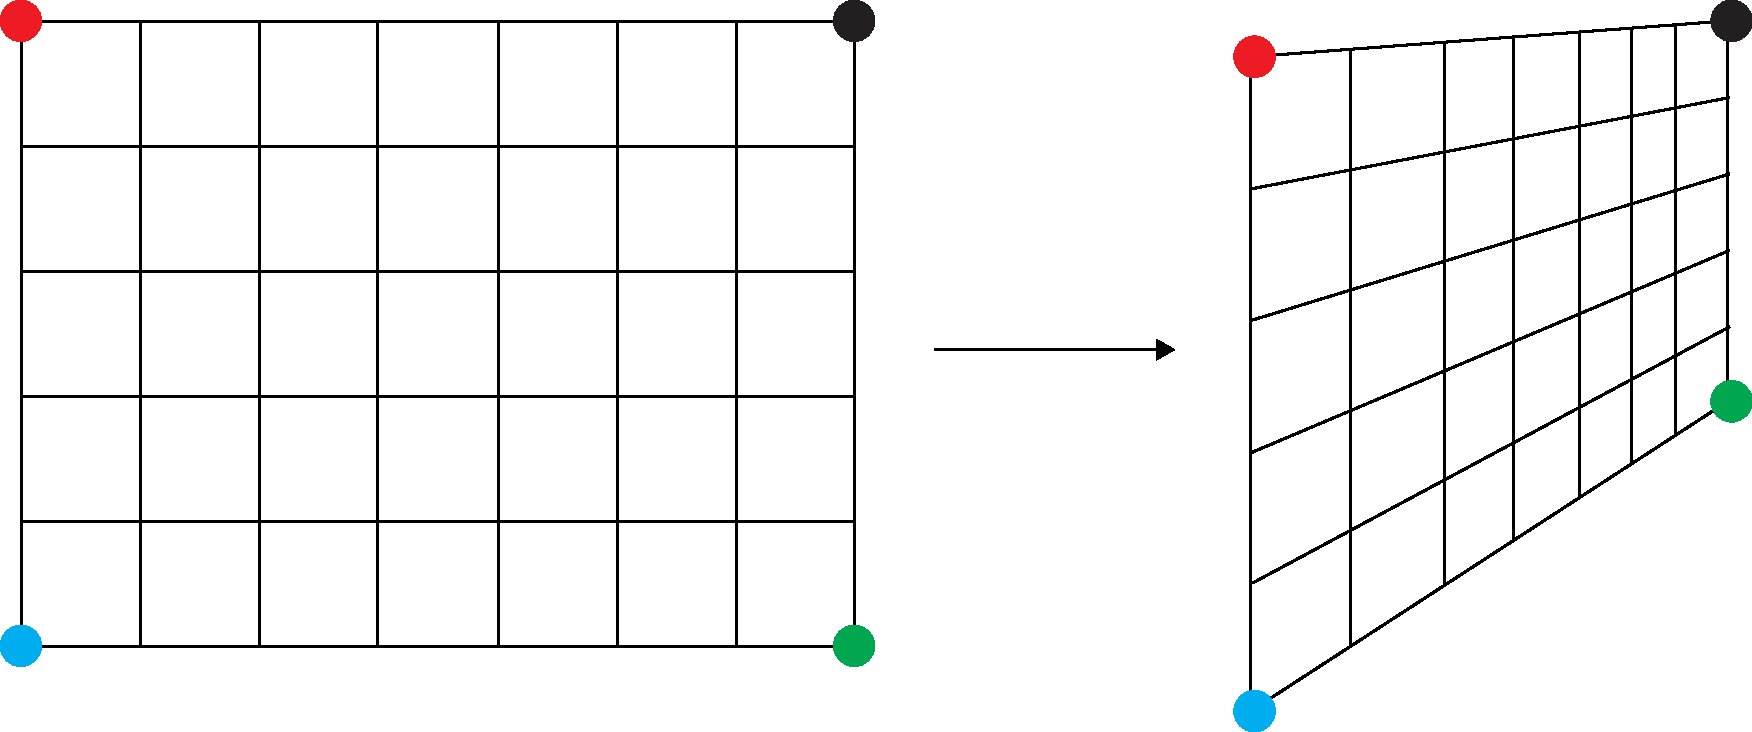
\includegraphics[width=\textwidth]{images/software/transformation/perspectiveTransformation.pdf}
\caption{Projective transformation}
\label{img:projectionGrid}
\end{center}
\end{figure}

Projective transformation are realised by simple matrix multiplication:
\begin{equation*}
\begin{pmatrix}
a_1 & a_2 & b_1  \\
a_3 & a_4 & b_2  \\
c_1 & c_2 & 1
\end{pmatrix}
\times
\begin{pmatrix}
x  \\
y  \\
1
\end{pmatrix}
=
\begin{pmatrix}
x'  \\
y'  \\
1
\end{pmatrix}
\end{equation*}

Where $a_1$ to $a_4$ is the rotational matrix which performs scaling and rotation, $t_1$ and $t_2$ is the translation vector, moving the content in space, and $c_1$ and $c_2$ is the projection vector. $x$ and $y$ are the source positions which are projected to $x'$ and $y'$.  

With the four prior calculated and transformed points it is possible to determine the projective transformation matrix so that the vertex of the content e.g. the widget with defined vertex points at position (0,0), (1,0), (0,1) and (1,1), are transformed to the calculated ones. 
The transformation of an exemplary clock widget as well as the projected rectified result is shown in~\autoref{img:SimpleWarpClock}. For calculating the transformation matrix the \textit{QTransformation} class provided by Qt was utilised. Calculation starting from the ground truth is done fully automatic without any interaction necessary by the user. 
\begin{figure}[htbp]
        \centering
        \begin{subfigure}[b]{0.27\textwidth}
                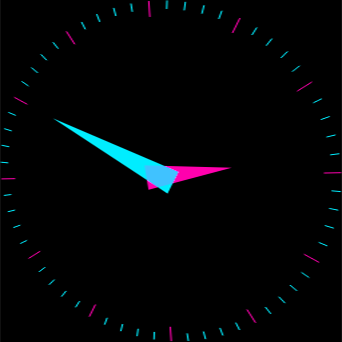
\includegraphics[width=\textwidth]{images/software/clock_3.png}
                \caption{Simple clock Widget}
                \label{img:SimpleWarpClock1}
        \end{subfigure}%
         \hfill 
         \begin{subfigure}[b]{0.27\textwidth}
                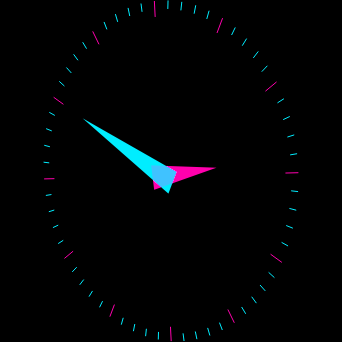
\includegraphics[width=\textwidth]{images/software/clock_warped.png}
                \caption{Pre-warped widget}
                \label{img:SimpleWarpClock2}
        \end{subfigure}
         \hfill
        \begin{subfigure}[b]{0.36\textwidth}
                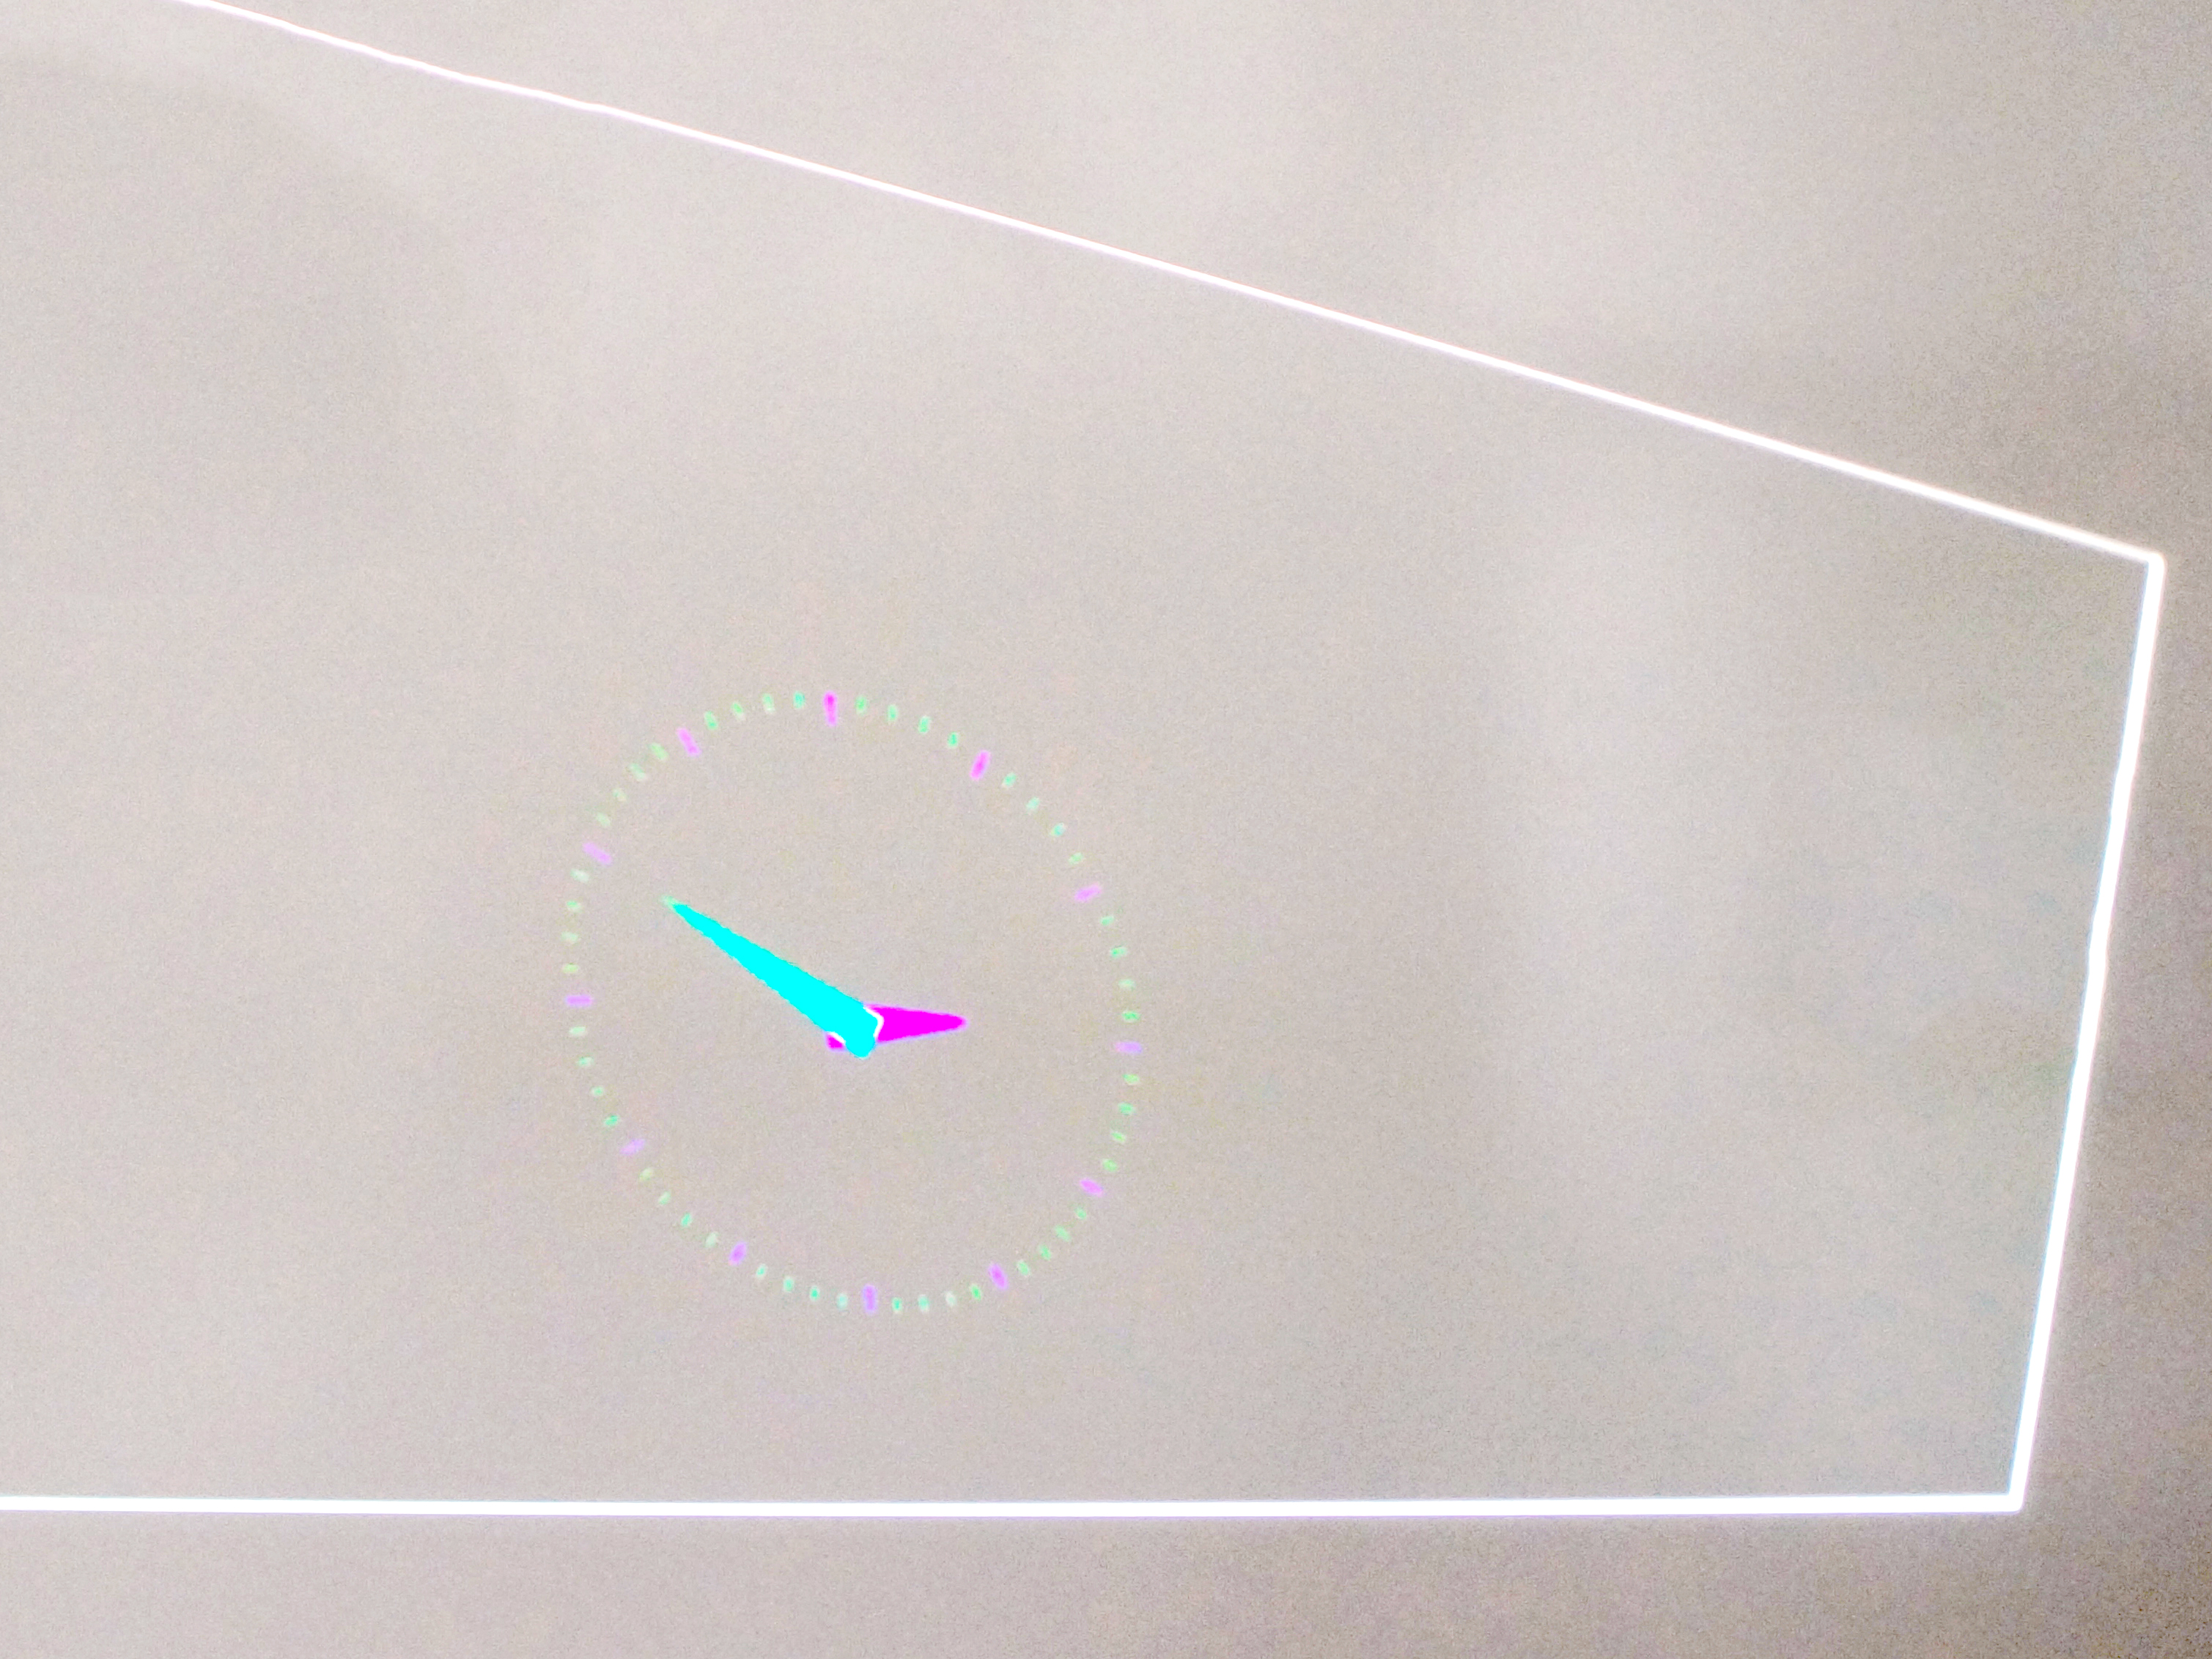
\includegraphics[width=\textwidth]{images/software/clock_project.jpg}
                \caption{Widget projected on surface}
                \label{img:SimpleWarpClock3}
        \end{subfigure}
        \caption{Pre-warping of a widget}\label{img:SimpleWarpClock}
\end{figure}

\pagebreak
\subsection{Widgets}\label{sec:widget}
The developed framework allows dynamic loading of widgets which actually displays the content to the user. 
All the complexity of the spatially aware projection, dynamic touch detection and movement of the PROCAMS are encapsulated and hidden from the view of the widget. This enables trouble-free and straight forward widget development. 

Two different possibilities are supported to create a new widget. Developers are able to implement the provided interface depicted in~\autoref{widgetCodeListing} to create a more desktop like looking widgets. The interface inherits from \textit{QWidget} the base class of all Qt user interfaces. The interaction logic can directly be implemented in the corresponding methods. In the \textit{paintEvent} method, the projected representation of the widget must be implemented. The core logic of the widget can be implemented as desired, for example by following the model view controller pattern.

Alternatively, developers can implement widgets using \ac{Qt Quick}. It uses QML to describe modern looking, fluid UIs in a declarative manner. Qt Quick is increasingly used on mobile phones or other embedded hardware.
QML allows to develop the logic using Javascript or even native code. Simplicity is shown by the source code (printed in~\autoref{QMLCodeListing}) for a plain widget showing a scrollable web page.
In both cases, widgets can easily be developed and tested in a common desktop environment by simply deploying them as a desktop application. This allows rapid creation of rich widgets without the need of the PROCAMS nearby. In addition, there are a lot of tutorials, demos and sample widgets provided by Qt Project \cite{Digia:BVAEvJrQ} which all run directly or after just small modifications in the framework.
\begin{figure}[htbp]
        \centering
        \begin{subfigure}[b]{0.235\textwidth}
                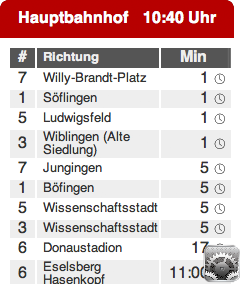
\includegraphics[width=\textwidth]{images/software/bus.png}
                \caption{Timetable widget}
                \label{img:wid:bus}
        \end{subfigure}
	\hfill
        \begin{subfigure}[b]{0.38\textwidth}
                \fbox{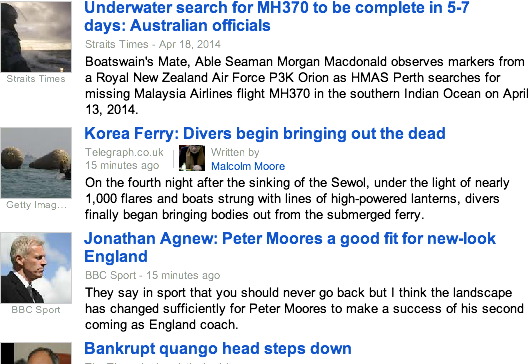
\includegraphics[width=\textwidth]{images/software/gnews.png}}
                \caption{Google News widget}
                \label{img:wid:news}
        \end{subfigure}
	\hfill
        \begin{subfigure}[b]{0.28\textwidth}
                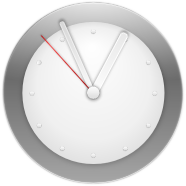
\includegraphics[width=\textwidth]{images/software/clock.png}
                \caption{Qt clock widget}
                \label{img:wid:time}
        \end{subfigure}
        \caption{Some implemented widgets}
        \label{fig:Widgets}
\end{figure}

Three widgets were implemented. A simple digital image frame which shows dynamically loaded images. On touching the left or right part of the image, the next or previous image is presented. The second widget is an adaptive bus time table (see~\autoref{img:wid:bus}) which shows the next buses leaving a desired bus stop. The last implemented widget is a news browser (see~\autoref{img:wid:news}), showing the Google news website. Any other web page could be displayed by this widget as well.
In addition, three widgets provided as demos by Qt Project were slightly modified to work with the proposed framework. The first one is a simple clock showing the time (see~\autoref{img:wid:time}), the second one is a sophisticated image browser allowing to browse the flickr.com image library in a convincing way. The third adapted widget shows a Twitter feed. There are many more examples available offering great services. Most of them can directly deployed into the developed framework. The three exemplary chosen widgets conduce just as proof of concept.